\chapter{Evaluation}

This chapter presents a complete evaluation of the application using three methods: \textbf{User Testing}, \textbf{Individual Interviews}, and the \textbf{User Experience Questionnaire (UEQ)}. The combination of these evaluation methods is intended to capture an overall view of the app’s usability, user engagement, effectiveness, and its ability to accurately depict the mood of students. Each method provides a unique perspective, ensuring that we can identify the application’s strengths and uncover any potential areas for improvement.\vspace{5mm} \\
Additionally, by combining \textbf{User Testing} and \textbf{Individual Interviews}, we aim to understand whether the application can capture the students' actual mood states. The interviews allow us to validate the observed user behavior and responses during the testing phase. This deeper understanding will help us evaluate how well the application fulfills its primary objective of accurately tracking the mood of students.\vspace{5mm} \\
The following overview explains the purpose of each evaluation method:

\begin{itemize}
    \item \textbf{User Testing}: This method helps us observe how participants interact with the application in a real-world context. By having users engage with the app over a period of time, we are able to assess the app’s usability, user engagement, and the general effectiveness of its features in meeting user needs. Additionally, it provides initial data about the participants' recorded moods, which we can later compare with their feedback from the interviews.

    \item \textbf{Individual Interviews}: Following the user test, we conduct interviews to gain detailed qualitative insights. This method allows us to explore users’ thoughts, experiences, and suggestions in more depth, providing context to the observations made during the user test. By discussing their moods during the user testing phase, participants can confirm or disprove the accuracy of the data collected, helping us understand if the application effectively captures their actual emotional states.

    \item \textbf{User Experience Questionnaire (UEQ)}: The UEQ offers a quantitative approach to evaluating the application’s user experience. This structured evaluation provides numerical insights into how users perceive various aspects of the application, validating findings from the previous two methods and providing a clear picture of user satisfaction.
\end{itemize}

\noindent The combination of these three evaluation methods allows us to integrate both qualitative and quantitative data, which can help us make decisions about necessary improvements and ensure that the final product delivers a meaningful and engaging experience for the users. The sections that follow dig into the procedures, results, and analysis defined for each method.

\section{User Test}

The testing phase of the application involved engaging a group of selected test users from a convenience sample, primarily consisting of friends and relatives, to validate the app's functionalities and user experience. Approximately 20 individuals were initially contacted, all of whom were students. Out of these, 9 participants expressed their willingness to be involved in the testing phase, which spanned over a period of approximately three weeks.
\begin{itemize}
    \item 7 of them are students in the University of Patras, Greece.
    \item 1 of them is student in the Agricultural University of Athens, Greece.
    \item 1 of them is student in the Karlsruhe Institute of Technology, Germany.
\end{itemize}
The following sections provide an overview of the instructions provided to the users, the testing procedure,a summary of feedback received during this phase and analysing the data results.

\subsection{Instructions}

The test users were given clear instructions on how to set up and use the application. They were asked to
\begin{enumerate}
    \item Download the Expo Go (or Expo) application \\
    from either the App Store (for iOS users) or Google Play Store (for Android users) respectively, as Expo Go is required to run React Native applications built with the Expo framework.\vspace{5mm} \\
    Once they installed the application, they were instructed to
    \item Connect by scanning the provided QR code or clicking on the URL link that I shared
\end{enumerate}

\noindent The test users were then briefed on the main functionalities of the app, specifically focusing on
\begin{itemize}
    \item Selecting their welcome mood
    \item Completing the ``Today's Survey''
\end{itemize}
\noindent and in general interact with the application. They were advised to perform these tasks daily, either immediately after receiving the notification that a new survey had been created or at a later time during the same day. If they were unable to complete the survey on the same day, they were told that they could still submit their responses within the following days. The users were also informed that this was a testing phase, and they might encounter some bugs or minor issues. For any major issues, such as the application failing to create a survey or notifications not being sent, users were instructed to report these problems immediately for prompt resolution. In the event of significant issues, a second round of testing would be scheduled to ensure all problems were addressed.

\subsection{Procedure}

The testing phase was from 5/9/2024 and finished on 26/9/2024. During this period, the users successfully followed the provided instructions and started using the application without reporting any major issues. Minor issues were reported, mostly related to Android-specific inconsistencies such as missing fonts and shadow effects that were not rendering correctly. These malfuctions were likely due to the fact that the front-end development was primarily conducted on an iPhone, which limited visibility into Android-specific bugs. Nevertheless, precautionary measures taken during development minimized these cross-platform issues.\vspace{5mm} \\
In addition to addressing the minor bugs reported, several improvements were made to the app's user interface, such as refining colors and adjusting component sizes to ensure a more consistent look and feel across devices. Throughout the testing period, all critical functionalities, including survey creation, mood tracking, and notifications, performed as expected, and the feedback from the users was positive. This confirmed that the application was stable enough for real-world usage.\vspace{5mm} \\
To keep the testing experience as unbiased as possible, I avoided giving the users any direct assistance or guidance on how to use the application. I wanted them to explore and understand the app's features independently, simulating a real-world user experience. While I did receive a few messages from users asking for clarification or reporting initial confusion, I encouraged them to save their feedback for the post-testing interviews. Some users also mentioned encountering minor issues during their first few minutes of usage, but after spending about 5-10 minutes with the app, they were able to navigate and use it without further complications.

\subsection{Participants' Exam Schedule}

During the three-week testing phase, it’s essential to consider that several participants were undergoing university exams, which could have influenced their mood and survey scores. The exam schedule varied in difficulty and frequency for each participant, adding a layer of context to the data collected:

\begin{itemize}
    \item \textbf{User 1}: Had three difficult courses scheduled on the 7th, 11th, and 18th of September.
    \item \textbf{User 2}: Managed a mix of three difficult courses (2nd, 9th, and 25th of September) and two easy courses (4th and 10th of September).
    \item \textbf{User 3}: Had no exams during this period, which likely contributed to a more stable mood and consistent engagement compared to the other participants.
    \item \textbf{User 4}: Had no exams during this period, same as ``User 3''.
    \item \textbf{User 5}: Had a packed schedule with four intermediate courses (29th of August, 5th, 10th, and 14th of September) and one difficult course on the 6th of September.
    \item \textbf{User 6}: Faced two intermediate courses on the 6th and 7th of September.
    \item \textbf{User 7}: Only had one easy course on the 7th of September, indicating that his schedule was relatively light.
\end{itemize}

\noindent The other participants weren't asked about their schedule because they eventually didn't participate in the testing phase.\vspace{5mm} \\
Understanding the participants' exam schedules provides valuable insight into their mental states and behavior during the testing phase, as academic stress could significantly influence their mood and survey responses. This context helps us interpret the results more accurately, especially for those participants with more demanding schedules.

\subsection{Results}

After completing the testing phase, I collected and analyzed the data submitted by users, focusing on their survey scores and initial welcome moods. This data was used to assess user engagement and interactions with the application. To further validate these findings, I cross-referenced them with feedback obtained from follow-up interviews to determine whether the application was used as intended. It was found that 7 out of 9 participants actively interacted with the application over a three-week period, though their usage varied and was not always consistent on a daily basis. Additionally, a few participants joined the testing phase later than the initial start date. Below is a summary of the data gathered from all participants throughout the testing period.

\vspace{5mm}

\noindent \textbf{Welcome Moods} \\
The welcome moods of the participants provide insight into their mental state and overall well-being during the testing phase. Each participant was asked to log their mood daily by choosing from several options, including ``nothing'', ``awful'', ``sad'', ``neutral'', ``good'' and ``happy''. These responses were then collected and analyzed to identify any trends or patterns. As shown in the mood distribution charts, participants exhibited varying emotional states, which were likely influenced by external factors such as their academic schedules, that we mentioned before.

\vspace{5mm}

\FloatBarrier
\begin{figure}[h!]
    \centering
    \subfloat[User 1]{%
        \begin{tikzpicture}
            \pie[text=legend, color={moodNothing, moodNeutral, moodGood, moodHappy}, radius=2, sum=auto, text=pin, explode={0.1, 0.1, 0.1, 0.1}]{
                28.57/nothing, 
                14.29/neutral, 
                35.71/good, 
                21.43/happy
            }
        \end{tikzpicture}
        \label{fig:`User 1'-welcome-mood}
    }
    \hfill
    \subfloat[User 2]{%
        \begin{tikzpicture}
            \pie[text=legend, color={moodNothing, moodGood, moodHappy}, radius=2, sum=auto, text=pin, explode={0.1, 0.1, 0.1}]{
                47.37/nothing, 
                21.05/good, 
                31.58/happy
            }
        \end{tikzpicture}
        \label{fig:`User 2'-welcome-mood}
    }
\end{figure}
\FloatBarrier

\FloatBarrier
\begin{figure}[h!]\ContinuedFloat
    \centering
    \subfloat[User 3]{%
        \begin{tikzpicture}
            \pie[text=legend, color={moodNothing, moodNeutral, moodGood}, radius=2, sum=auto, text=pin, explode={0.1, 0.1, 0.1}]{
                70.0/nothing, 
                10.0/neutral, 
                20.0/good
            }
        \end{tikzpicture}
        \label{fig:ioannis-welcome-mood}
    }
    \hfill
    \subfloat[User 4]{%
        \begin{tikzpicture}
            \pie[text=legend, color={moodNothing, moodSad, moodNeutral, moodGood}, radius=2, sum=auto, text=pin, explode={0.1, 0.1, 0.1, 0.1}]{
                42.86/nothing, 
                4.76/sad, 
                33.33/neutral, 
                19.05/good
            }
        \end{tikzpicture}
        \label{fig:`User 4'-welcome-mood}
    }
\end{figure}
\FloatBarrier

\FloatBarrier
\begin{figure}[h!]\ContinuedFloat
    \centering
    \subfloat[User 5]{%
        \begin{tikzpicture}
            \pie[text=legend, color={moodNothing, moodNeutral, moodGood, moodHappy, moodSad}, radius=2, sum=auto, text=pin, explode={0.1, 0.1, 0.1, 0.1, 0.1}]{
                22.72/nothing, 
                18.18/neutral, 
                45.45/good, 
                9.09/happy,
                4.54/sad
            }
        \end{tikzpicture}
        \label{fig:`User 5'-welcome-mood}
    }
    \hfill
    \subfloat[User 6]{%
        \begin{tikzpicture}
            \pie[text=legend, color={moodNothing, moodGood, moodHappy}, radius=2, sum=auto, text=pin, explode={0.1, 0.1}]{
                84.21/nothing, 
                10.53/good, 
                5.26/happy
            }
        \end{tikzpicture}
        \label{fig:`User 6'-welcome-mood}
    }
\end{figure}
\FloatBarrier

\FloatBarrier
\begin{figure}[h!]\ContinuedFloat
    \centering
    \subfloat[User 7]{%
        \begin{tikzpicture}
            \pie[text=legend, color={moodNothing, moodGood, moodHappy}, radius=2, sum=auto, text=pin, explode={0.1, 0.1, 0.1}]{
                81.82/nothing, 
                9.09/good, 
                9.09/happy
            }
        \end{tikzpicture}
        \label{fig:yiannis-welcome-mood}
    }
    \caption{Mood Distribution for Each User}
\end{figure}
\FloatBarrier

\vspace{5mm}

\noindent \textbf{Questionnaire Scores} \\
The figure below illustrates the scores obtained by each participant across different survey instances during the testing phase. Each colored bar represents the score of a specific survey, identified by its corresponding survey number in the legend. The height of the bars indicates the score achieved, with a maximum value of 26 for each survey. The x-axis displays the dates of each survey, while the y-axis shows the score values.\vspace{5mm} \\
This visualization provides an overview of the survey completion and engagement of each participant. Gaps or missing bars indicate periods when the participant did not complete a survey. This could be due to a variety of reasons, such as forgetting to take the survey, lack of time, or disinterest. Also a one day gap is natural, because the user finishes the survey, and the next day anew survey is being created. Additionally, variations in scores across surveys reflect the changes in participants' responses, potentially influenced by factors like daily mood fluctuations or external stressors, such as exams.

\vspace{5mm}

\FloatBarrier
\begin{figure}[ht]
    \centering
    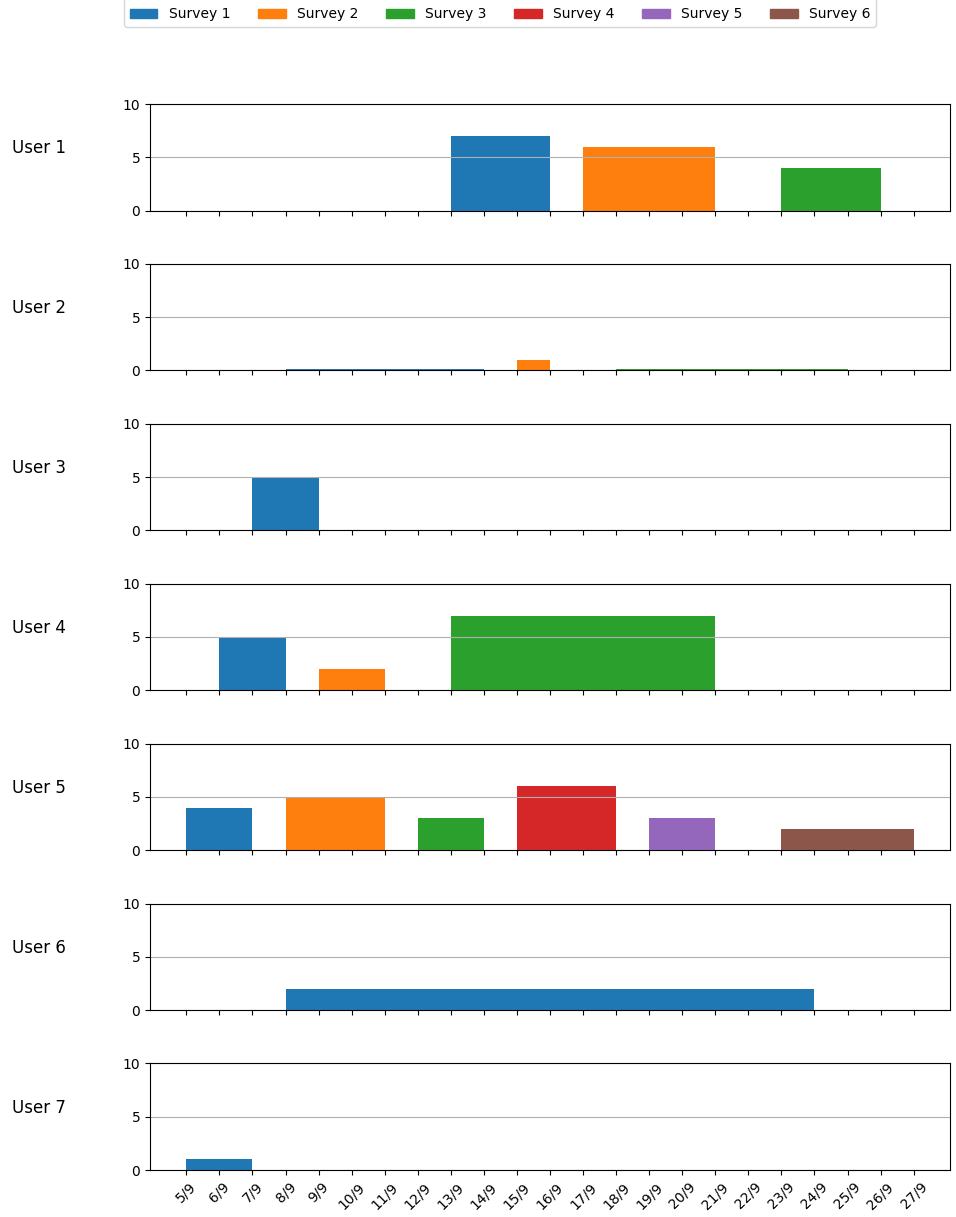
\includegraphics[width=\linewidth]{figures/Figure-Scores.png}\label{fig:questionnaire-results}
    \caption{Questionnaire Results of the test users}
\end{figure}
\FloatBarrier

\vspace{5mm}

\subsection{Conclusion}

The results obtained during the testing phase show a diverse range of interactions and emotional responses from the participants, heavily influenced by their exam responsibilities. Participants with a more demanding exam schedule, such as \textbf{User 1} and \textbf{User 2}, exhibited higher frequencies of ``nothing'' and ``neutral'' welcome moods, indicating potential stress or lack of engagement during high-pressure periods. This trend is further supported by their questionnaire scores, which show considerable variability across different surveys, likely reflecting the fluctuations in their mental state as they navigated through challenging exams.\vspace{5mm} \\
Conversely, participants like \textbf{User 3} and \textbf{User 4}, who did not have any exams during the testing period, demonstrated more stable welcome mood distributions and consistent engagement in the daily surveys. This stability is echoed in their questionnaire scores, which did not exhibit the same level of fluctuation as those with heavier academic responsibilities.\vspace{5mm} \\
Interestingly, \textbf{User 5} and \textbf{User 6}, who faced a mix of intermediate and difficult courses, showed a more balanced distribution of welcome moods, with fewer ``nothing'' days compared to \textbf{User 1} and \textbf{User 2}. Their survey scores also reflect this balance, with some variations that indicate the challenges of their schedules without reaching the extremes seen in other participants.\vspace{5mm} \\
Additionally, it’s worth noting that several participants showed limited engagement with the application. This lack of engagement is evident in the frequency of “nothing” welcome moods and the low completion rates of the daily surveys. These findings suggest that participants may have been too occupied to fully engage with the app, highlighting the importance of addressing user motivation and commitment, especially during busy periods.\vspace{5mm} \\
Overall, the data points to a strong link between exam stress and mood, demonstrating how external factors can significantly impact emotional well-being and participation levels. By considering these factors, we can gain better insights into user behavior and adjust the application to offer more personalized support during high-stress times. This can ultimately make mood tracking more effective and reliable, catering better to users’ varying levels of engagement.
Overall, there is a clear link between exam stress and mood, as seen in many participants. This shows how external factors can significantly influence emotional well-being and survey responses. By considering these relationships, we can better understand the data and see how academic stress affects mood and participation. These insights help us improve the application to better support users during stressful times and make mood tracking more accurate and effective.

\section{Interviews}

To validate the conclusions drawn from the testing phase and gain deeper insight into the participants’ experiences with the application, individual interviews were conducted with each user. The purpose of these interviews was to explore their perspectives on the app's usability, overall experience, and its ability to accurately reflect their emotional states. By discussing about their moods during the user test phase, these interviews allowed us to confirm whether the application successfully depicted the participants’ actual moods and provided meaningful support for managing their well-being.

\subsection{Procedure}

During the testing phase, 7 out of the 9 participants actively used the application. However, only 6 participants were available for an interview, all except `User 3', and their feedback was gathered to gain a deeper understanding of their experiences with the app. A structured set of questions was prepared to cover a wide range of topics, including usability, user satisfaction, and areas of potential improvement. The questions aimed to gather feedback on various functionalities of the application and determine if it met the users' expectations. The questions asked during the interviews were as follows:

\begin{enumerate}
    \item \textbf{First impressions}: What were your initial thoughts before using the application? Was there any feature that stood out or surprised you, either positively or negatively?
    \item \textbf{Usage environment}: Where did you primarily use the application (e.g., at home, outdoors)? How would you describe your past three weeks—were they more stressful or relaxed?
    \item \textbf{Emotional impact}: How did you feel before and during the usage of the application? Did you feel obliged to use it, or was it something you engaged with naturally?
    \item \textbf{Ease of use}: Did you encounter any difficulties while using the app? Were there aspects that felt particularly challenging or, on the contrary, very straightforward?
    \item \textbf{Previous experience}: Have you used any similar applications in the past? If so, how would you compare your experience?
    \item \textbf{Feature feedback}: What features do you think are missing, or which ones require modifications?
    
    \vspace{2mm} If the participant did not address specific features, additional follow-up questions were asked:

    \begin{itemize}
        \item Was the content of the questionnaire appropriate and relevant?
        \item How did you feel about the questionnaire process and the frequency with which questions were repeated?
        \item Did you find the notifications helpful, or do you feel something was lacking?
    \end{itemize}
    
    \item \textbf{Frequency of use}: How often do you think you would use this application in your daily life?
    \item \textbf{Application summary}: How would you describe the application in one sentence or just a few words?
    \item \textbf{Additional comments}: Is there anything else you would like to add that we haven’t discussed?
\end{enumerate}

\noindent These questions provided a comprehensive view of the participants’ experiences and gathered valuable feedback to refine the application further.

\subsection{User Perspectives}

Based on the feedback collected from the user interviews, we can pinpoint various aspects of the application that users either appreciated or found areas for improvement.

\begin{enumerate}
    \item \textbf{First Impressions}
\end{enumerate}

\noindent Most participants were impressed by the design and interface of the application. Several users, like `User 1' and `User 2', highlighted the animation and visuals as a key feature that initially caught their attention. `User 4' mentioned that the immediate start of the welcome mood selection felt a bit abrupt but overall liked the simple and engaging interface. `User 6' described the design as ``really good'' and appreciated the quick loading time.

\begin{enumerate}[resume]
    \item \textbf{Usage Environment}
\end{enumerate}

\noindent Participants mainly used the application at home, with only a few trying it in other environments, such as cafés or while taking a walk. This pattern is primarily due to the exam period that many of them were going through, which limited their movement outside. For example, `User 2' used it at home 90\% of the time, while `User 5' occasionally used it outdoors.

\begin{enumerate}[resume]
    \item \textbf{Emotional Impact}
\end{enumerate}

\noindent The general aggrement between the users was that the application did not feel like an obligation or chore. However, `User 4' and `User 5' noted that as the days passed, the repetitive nature of the questions became a bit boring, making it feel less engaging over time. Participants like `User 7' found the app useful but felt that better use of data could enhance its impact on their mood management.

\begin{enumerate}[resume]
    \item \textbf{Ease of Use}
\end{enumerate}

\noindent Users found the application easy to navigate with clear guidance and large buttons. `User 1' described it as ``really simple, easy to use, and operational'', while `User 4' and `User 6' highlighted minor confusion at certain points, such as accidentally retaking surveys or understanding the purpose of some buttons. These initial usability issues resolved themselves with continued use.

\begin{enumerate}[resume]
    \item \textbf{Previous Experience}
\end{enumerate}

\noindent Most participants had not used similar applications before, making this their first exposure to a mood-tracking app. For example, `User 2' noted that he enjoyed the experience as it made him reflect on his day, something he wouldn’t usually do. `User 4' mentioned he wanted to use a similar app before, but the subscription-based nature discouraged him.

\begin{enumerate}[resume]
    \item \textbf{Feature Feedback}
\end{enumerate}

\noindent While most users appreciated the features, some specific recommendations were made for improvement:

\begin{itemize}
    \item \textbf{Questionnaire Content:} Several users felt that some of the questions were too extreme or repetitive. For instance, `User 5' and `User 7' suggested more general questions related to daily life rather than intense psychological states. `User 4' recommended a mix of certified and custom questions to keep the content balanced and engaging.

    \item \textbf{Survey Process and Frequency:} Some participants, such as `User 2', felt that the survey could be available earlier in the day, allowing more flexibility in responding. On the other hand, `User 1' suggested that the application should create the survey and notify the user during the evening, to better depict the user's overall daily mental health. `User 4' suggested adding a new question each day or refreshing the question set every few days to prevent monotony.

    \item \textbf{Notifications:} Notifications were generally appreciated for keeping users engaged. However, `User 1' and `User 4' suggested making them more personalized or playful, such as including emojis or varying text content.

    \item \textbf{Message Feature (Quotes/Advice):} The message feature received positive feedback for its motivational aspect, though users like `User 5' mentioned that at times the text color clashed with the background, making it hard to read.

    \item \textbf{Statistics:} There was some confusion around the bar chart, especially regarding the scores displayed. Participants were unsure about the meaning of low scores until it was explained to them. This highlighted a need for clearer communication of the results and scores.
\end{itemize}

\noindent The users also were asked about new features that they would like to see, so they proposed some ideas such as:

\begin{itemize}
    \item \textbf{Diary Feature:} `User 4' and `User 6' both suggested introducing a diary feature where users could write down their thoughts or capture daily insights, further enhancing the app's role as a personal mood tracker and journal.

    \item \textbf{Photo-Based Mood Capture:} `User 6' also proposed adding a feature similar to ``BeReal'' where users could capture and upload a photo every day to visually document their emotions, adding an additional dimension to mood tracking.

    \item \textbf{Gamification Elements:} Some participants suggested incorporating more gamification elements to make the experience more engaging. For example, `User 1' mentioned introducing streaks or achievements based on consistent usage, while `User 6' suggested including daily or weekly challenges that encourage user participation.

    \item \textbf{Adaptive Questionnaire Content:} Another suggestion was to implement adaptive questionnaires that adjust based on the user’s responses or history, gradually becoming more tailored to their personal experiences and mental state. This would ensure that the content remains relevant and engaging over time.
\end{itemize}

\begin{enumerate}[resume]
    \item \textbf{Frequency of Use}
\end{enumerate}

\noindent Participants expressed varied interest in using the application regularly. Those without exams or stressful schedules, such as `User 7' and `User 4', felt they could use the application daily. However, participants like `User 5' mentioned they might reduce their usage during exam periods due to time constraints.

\begin{enumerate}[resume]
    \item \textbf{Application Summary}
\end{enumerate}

\noindent Each user summarized the application in their own unique way, highlighting different aspects of their experience. `User 1' described it simply as ``My diary!'', emphasizing its role in tracking his day-to-day emotions. `User 6' offered a more detailed description, calling it: ``Delightful, innovative, and pioneering, which is well designed and constructed''. `User 4' viewed the app as ``Playful and engaging'', noting its potential for daily use if some improvements were made. `User 2' described it as ``Emotion'', reflecting how the app made him more aware of his mental state. `User 5' referred to it as ``Simple, accessible, and straightforward'', praising its user-friendly interface. `User 7' appreciated its potential value for mental health, describing it as ``Useful and promising''. Each participant's summary captures a different perspective, showcasing the diverse ways the application impacted their experience.

\begin{enumerate}[resume]
    \item \textbf{Additional Comments}
\end{enumerate}

\noindent No more comments, from the users, about the application, so the users were given the chance to ask any questions they had about the app, leading to insightful discussions about its features and potential future enhancements. Several participants expressed curiosity about different aspects of the app, such as its deployment process, the scoring system, and the possibility of adding new functionalities. This engagement provided a deeper understanding of how users perceived the app and what additional features they felt would improve their overall experience. For instance, `User 1' was interested in learning whether the application could evolve with new features based on user feedback. `User 5', on the other hand, was curious about the technical deployment process and the tools used, such as Docker and Google Cloud. `User 2' and `User 6' wanted clarification on how the questionnaire scores were calculated and how they correlated with their mental state. These discussions helped clarify certain functionalities and revealed areas for further development, making it clear that users were invested in understanding the application on a more detailed level.

\subsection{Conclusion}

The interviews provided valuable insight into how users perceived and interacted with the application. Across the nine different topics discussed, participants shared a mix of positive feedback and constructive suggestions for improvement. They appreciated the application's simple and intuitive design, its motivational message feature, and the ease of navigating the survey process. However, many pointed out areas that could be improved, like offering a wider range of questions, changing the timing and format of notifications, and allowing more flexibility with the survey schedule. Additionally, users highlighted the need for clearer communication of survey scores and results to enhance understanding of their mood trends over time.\vspace{5mm} \\
The interviews also confirmed that the application was generally successful in depicting participants’ actual moods during the testing phase. Although it did not capture their emotional states with complete accuracy, the app’s assessments were considered to be reflective of users' real moods  most of the times. This finding highlights the application’s potential as a reliable mood-tracking tool, while also emphasizing the importance of including more personalized elements to further enhance its accuracy.\vspace{5mm} \\
Suggestions for additional features, such as incorporating a diary or photo-based mood tracking option, were common among several users and indicate a desire for more personal and expressive ways to document their emotional states. The feedback on the questionnaire content, particularly the call for more balanced and less extreme questions, suggests an opportunity to make the app feel more relatable and less formal.\vspace{5mm} \\
Overall, the interviews strengthen the value of the application while shedding light on key areas for improvement. The insights gathered are important in guiding the next steps for development, ensuring that the application continues to meet user needs and provide meaningful support for mental health and well-being.

\section{UEQ Questionnaire}

To get a more complete evaluation of the application, I included the UEQ questionnaire. While the interviews provided good qualitative feedback, I needed a quantitative measure (with numbers) to confirm that users had a positive experience. The UEQ helped validate these results by capturing key aspects of the user experience in a structured way.\vspace{5mm} \\
The \textbf{\href{https://www.ueq-online.org/}{User Experience Questionnaire (UEQ)}}\footnote{\url{https://www.ueq-online.org/}} is a widely used tool for evaluating the user experience of interactive products. It offers valuable insights into how users perceive an application’s usability and user interface, by measuring six distinct dimensions: Attractiveness, Perspicuity, Efficiency, Dependability, Stimulation, and Novelty. These dimensions provide insights into both the pragmatic qualities (such as how easy it is to use the application) and hedonic qualities (such as how engaging or motivating the app is).

\subsection{Procedure}
For the evaluation of the application, six out of the nine user testers who participated in the previous testing phase and in the interviews phase were selected. These participants were chosen based on their level of engagement and consistent use of the application throughout the testing period. The remaining three participants were excluded from this evaluation due to their minimal usage and interaction with the application.\vspace{5mm} \\
The procedure for conducting the UEQ was straightforward and designed to minimize complexity for the participants. A Google Form was created, containing all the questions from the UEQ. This format was chosen to ensure that the questionnaire could be completed quickly and easily, without imposing additional time constraints on the users. The Google Form link was then shared with each participant through direct messages on various platforms such as Instagram, Messenger, and WhatsApp. This approach facilitated efficient communication and allowed participants to complete the questionnaire at their convenience.

\subsection{Results}
Based on the results provided by the UEQ questionnaire, we can derive some key insights about the user experience of the application. The UEQ measures different aspects of user experience using a variety of scales such as Attractiveness, Perspicuity (ease of understanding and learning), Efficiency, Dependability, Stimulation, and Novelty. So the concluding text for each of the scales is shown below:

\begin{enumerate}
    \item \textbf{Overall Attractiveness}: The responses indicate that the application is generally considered attractive by the users. This suggests a positive perception of the application's visual design, layout, and overall appeal.
    \item \textbf{Perspicuity (Ease of Use)}: Participants rated the application as understandable and easy to learn, indicating that users did not struggle with comprehending the features or navigation. This suggests that the application is intuitive and well-organized.
    \item \textbf{Efficiency}: Users considered the application efficient, which reflects that they felt it was effective in achieving its purpose without unnecessary complexity or time wastage.
    \item \textbf{Dependability}: The scores show that the users found the application dependable. This dimension is associated with users' perceptions of control, security, and predictability of the application.
    \item \textbf{Stimulation (Excitement and Engagement)}: The results were mixed for this category, suggesting that while some users found the application stimulating and engaging, others found it somewhat repetitive. This could be linked to the feedback from interviews about the need for more variety in the questionnaires or features.
    \item \textbf{Novelty (Innovation and Creativity)}: The novelty scores suggest that the application was seen as somewhat conventional. Users appreciated its innovative elements but may have felt that additional creative features or more dynamic interactions could further enhance their experience.
\end{enumerate}

\subsection{Conclusion}
The UEQ results validate the findings from the interviews by confirming that the application is user-friendly, easy to understand, and visually appealing. However, there is room for improvement in the areas of stimulation and novelty. Introducing new features, varying the questions, or adding interactive elements could address these aspects, making the application more engaging and less repetitive.

\section{Discussion}

The evaluation using \textbf{User Testing}, \textbf{Individual Interviews}, and the \textbf{User Experience Questionnaire (UEQ)} provided a complete view of the application's performance, usability, and effectiveness in meeting its primary objective. Each method revealed key insights into how the application supports students in tracking and managing their mood.

\subsection{Overall Findings}

The \textbf{User Testing} phase showed that participants were generally able to interact with the app independently after a short learning period, highlighting its ease of use and accessibility. Despite minor issues, the overall experience was positive, confirming the app's usability.\vspace{5mm} \\
The \textbf{Interviews} validated that the application captured participants’ moods accurately most of the time. Users appreciated its simple design but suggested enhancements such as adding a diary feature or more diverse content to better reflect their emotional states. These suggestions indicate that while the app performs well, additional personalization would improve its effectiveness.\vspace{5mm} \\
The \textbf{UEQ} results comfirmed these observations, showing high scores in usability and attractiveness but lower scores in engagement and novelty. This suggests that while the app is user-friendly and functional, there is room for improvement in keeping users engaged over time.

\subsection{Achievement of Primary Objective}

The primary objective, which was mentioned in the first chapter, was to create a tool that helps students track their mood and manage their well-being. The evaluation confirms that the app achieved this goal by providing a platform for mood tracking and reflection. Although it didn’t capture moods with complete accuracy, the application was able to depict the users' emotional states in a high percentage of cases, making it a reliable tool for mood tracking.

\subsection{Areas for Improvement}

The evaluation highlighted areas for further development, including more adaptive questionnaires, a diary feature, and improved data visualization. Addressing these aspects could make the application more engaging and responsive to users’ needs.

\section{Conclusion}

The evaluation results confirm that the developed application successfully provides students with a practical tool for tracking their mood and well-being throughout their academic journey. Through the combined use of \textbf{User Testing}, \textbf{Interviews}, and the \textbf{UEQ}, the app demonstrated strong usability, an intuitive interface, and the ability to depict users' emotional states with reasonable accuracy. Although certain areas, such as engagement and personalization, require further refinement, the overall feedback suggests that the app has achieved its primary objective of supporting students' mental health. Moving forward, incorporating user suggestions and more adaptive features will be crucial to enhancing the app's impact and ensuring it remains a relevant and valuable tool for students.
